\documentclass[conference]{IEEEtran}
\IEEEoverridecommandlockouts
\usepackage{cite}
\usepackage{amsmath,amssymb,amsfonts}
\usepackage{graphicx}
\usepackage{textcomp}
\usepackage{xcolor}
\usepackage{booktabs}
\usepackage{microtype}
\usepackage{placeins}
\usepackage{balance}
\usepackage{url}
\usepackage{listings}
\lstset{basicstyle=\ttfamily\footnotesize,breaklines=true,columns=fullflexible,
  keepspaces=true,frame=single,rulecolor=\color{black!25},showstringspaces=false}
\newtheorem{proposition}{Proposition}
\usepackage{tikz}
\usetikzlibrary{arrows.meta,positioning,fit,backgrounds,calc}
\usepackage[hidelinks]{hyperref}
\newcommand{\R}{\mathbb{R}}
\newcommand{\override}{\texttt{DIGITAL\_TWIN\_OVERRIDE}}
\newcommand{\isolation}{\texttt{ASSET\_ISOLATION}}


\input{update_numbers.tex}
\begin{document}
\title{CommunityGuard-AI: Agentic AI for Cyber-Physical Defense of Energy Communities}

\author{
\IEEEauthorblockN{Maanat Bhadani, Alaa Selim, and Junbo Zhao}
\IEEEauthorblockA{
\textit{Thayer School of Engineering, Dartmouth College}\\
Hanover, NH, USA\\
\{maanat.h.bhadani.29, alaa.e.selim, junbo.zhao\}@dartmouth.edu
}
}
\maketitle


\begin{abstract}

Energy communities rely on accurate measurements to coordinate buildings, solar generation, and batteries. Detecting corrupted data is only the first step: a poor repair can introduce further errors. This paper presents CommunityGuard-AI, a four-stage framework that connects numerical evidence, incident diagnosis, repair planning, and verification. Its contribution is a complete response workflow that selects a repair tool, checks individual changes against peer references and a protected energy balance, and retains received data when no proposal passes verification. LangGraph manages execution, bounded retries, and decision records. A conditional proof states when an accepted change reduces measurement error. We evaluated the framework with rule-based decisions on two CityLearn building groups comprising \CaseN{} attacked records and \CleanN{} clean controls. It improved \ImproveN{} attacked records, left \UnchangedN{} unchanged, and worsened \HarmN{}, reducing mean normalized error by \ErrorReduction{}\%. \CleanAbstract{} A supplementary comparison examined Llama as the diagnosis and planning component. \PairedAbstract{} Actual responses, token counts, and processing times documented the language component's behavior and workload. The study demonstrated selective, traceable offline telemetry repair under explicit sensor-trust and reference-accuracy assumptions.

\end{abstract}

\begin{IEEEkeywords}
energy communities, telemetry repair, verification, agentic AI, cyber-physical security
\end{IEEEkeywords}
\section{Introduction}

Energy communities coordinate building demand, photovoltaic (PV) generation, battery energy storage systems (BESSs), and price-responsive devices through shared measurements. Their operation depends on knowing how much energy buildings consume, how much renewable generation is available, and when that energy is needed. Corrupted load, PV, price, or timing information can mislead the decisions that coordinate these resources, linking telemetry integrity to the cyber-physical security of distribution systems \cite{citylearnv2,khalaf2024survey}. Smart-inverter interfaces and synchronization signals provide concrete examples of this exposure \cite{mccarthy2024smartinverters,zhang2013time}.

Detecting an unusual value does not explain how to repair it. A false-data-injection attack can preserve realistic magnitudes and daily patterns \cite{liu2011false}. For example, an under-reported load can still follow its normal daily shape. The defender must identify the affected building and measurement channel, choose a reliable replacement, and avoid changing healthy data. A poor repair can add errors to the information supplied to a controller. The challenge is to connect detection to a limited, testable response.

Anomaly detectors address part of this challenge. Autoencoders learn normal patterns and identify deviations without labeled examples of every attack \cite{zideh2024aae}. However, their reconstructed values are estimates: a replacement can fit the model better while moving farther from the true measurement. Energy balance and measurements from other buildings provide additional checks. These checks depend on trusted sensors and accurate reference estimates. A repair method must state these assumptions, limit which values it changes, and keep the received data when the evidence is insufficient.

A complete response workflow must connect evidence to action while keeping proposed repairs subject to numerical checks. Large language models (LLMs) can contribute incident interpretation and tool selection \cite{majumder2024llm,liu2025agents}, although their diagnoses and explanations can be unsupported \cite{ruan2024threats}. Digital-twin and constrained-LLM studies have combined numerical evidence with language reasoning \cite{srivastava2024twins,kampourakis2026}. For telemetry defense, the central design question is how to organize diagnosis, repair tools, verification, and fallback behavior into a response whose effect can be measured independently.

CommunityGuard-AI addresses this question through four stages: numerical evidence, incident diagnosis, repair planning, and verification. The diagnosis and planning stages support rule-based or Llama decisions. Both use the same repair tools and numerical guard. LangGraph manages evidence requests, one allowed retry, accepted changes, and abstention (keeping the received data). Llama contributes language-based interpretation and tool selection within this structure. The framework's response conditions apply to either decision policy.

The paper makes three contributions: (i) an integrated response workflow that connects building/channel diagnosis to executable repair tools, selective changes, and bounded fallback; (ii) a verification rule using calibrated references and a protected energy balance, with a conditional proof of error reduction; and (iii) an evaluation on two building groups using later data for testing and withheld clean measurements for scoring. The evaluation measures recovery, errors introduced into healthy data, and failure cases. A supplementary Llama comparison examines language-based decisions, execution traces, token use, and latency within the same framework.

\section{System and Threat Model}

\subsection{Energy-Community Model}

We consider $N$ heterogeneous CityLearn buildings, indexed by $\mathcal{B}=\{1,\ldots,N\}$, with non-shiftable loads, PV generation, and electrical storage. Figure~\ref{fig:community} shows their observation flow.

\begin{figure}[t]
\centering
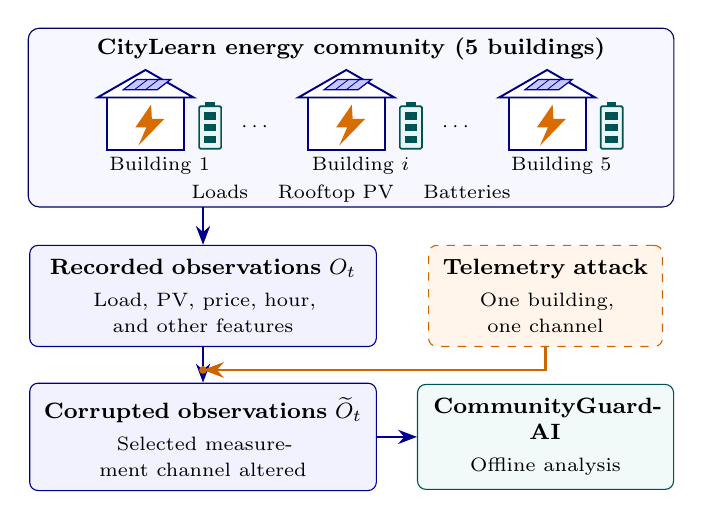
\begin{tikzpicture}[font=\footnotesize,>=Stealth,
 flow/.style={->,line width=0.85pt,draw=blue!55!black},
 box/.style={rounded corners=3pt,align=center,inner sep=5pt},
 house/.style={draw=blue!50!black,fill=white,line width=0.7pt}]
% Representative buildings within the five-building evaluation community.
\path[draw=blue!40!black,fill=blue!3,rounded corners=4pt]
  (0,3.85) rectangle (8.2,6.12);
\node[font=\footnotesize\bfseries] at (4.1,5.86)
  {CityLearn energy community (5 buildings)};
\foreach \x/\b in {1.55/1,4.10/i,6.65/5}{
  \begin{scope}[shift={(\x,4.57)}]
    \path[house] (-0.55,0) rectangle (0.43,0.67);
    \path[house] (-0.67,0.67)--(-0.06,1.02)--(0.55,0.67)--cycle;
    % Rooftop PV panel, drawn as a small blue module.
    \path[draw=blue!65!black,fill=blue!22,line width=0.45pt]
      (-0.34,0.77)--(0.09,0.77)--(0.26,0.90)--(-0.17,0.90)--cycle;
    \draw[blue!55!black,line width=0.3pt] (-0.20,0.77)--(-0.03,0.90)
      (-0.06,0.77)--(0.11,0.90);
    % Load symbol inside the building.
    \path[fill=orange!85!black] (0.01,0.58)--(-0.19,0.29)--(-0.05,0.29)
      --(-0.15,0.06)--(0.18,0.40)--(0.02,0.40)--cycle;
    % Battery beside the building.
    \path[draw=teal!65!black,fill=teal!8,rounded corners=0.5pt,line width=0.6pt]
      (0.62,0.02) rectangle (0.90,0.56);
    \path[fill=teal!65!black] (0.70,0.56) rectangle (0.82,0.61);
    \foreach \y in {0.09,0.24,0.39}
      \path[fill=teal!65!black] (0.68,\y) rectangle +(0.16,0.09);
    \node[font=\scriptsize] at (0.12,-0.20) {Building $\b$};
  \end{scope}
}
\node[font=\scriptsize] at (2.90,4.86) {$\cdots$};
\node[font=\scriptsize] at (5.45,4.86) {$\cdots$};
\node[font=\scriptsize] at (4.1,4.02) {Loads \quad Rooftop PV \quad Batteries};

\node[box,draw=blue!55!black,fill=blue!5,
 text width=4.05cm,minimum height=1.04cm] (clean) at (2.22,2.72)
 {\textbf{Recorded observations $O_t$}\\[2pt]
  {\scriptsize Load, PV, price, hour, and other features}};
\node[box,draw=orange!80!black,fill=orange!8,dashed,
 text width=2.62cm,minimum height=1.04cm] (attack) at (6.57,2.72)
 {\textbf{Telemetry attack}\\[2pt]
  {\scriptsize One building, one channel}};
\draw[flow] (2.22,3.85)--(clean.north);

\node[box,draw=blue!55!black,fill=blue!5,
 text width=4.05cm,minimum height=0.96cm] (corrupt) at (2.22,0.93)
 {\textbf{Corrupted observations $\widetilde{O}_t$}\\[2pt]
  {\scriptsize Selected measurement channel altered}};
\node[box,draw=teal!65!black,fill=teal!5,
 text width=2.90cm,minimum height=0.96cm] (analysis) at (6.57,0.93)
 {\textbf{CommunityGuard-AI}\\[2pt]
  {\scriptsize Offline analysis}};
\draw[flow] (clean.south)--(corrupt.north);
\draw[->,line width=1pt,draw=orange!80!black]
  (attack.south)--(6.57,1.78)--(2.22,1.78);
\fill[orange!80!black] (2.22,1.78) circle (1.4pt);
\draw[flow] (corrupt.east)--(analysis.west);
\end{tikzpicture}
\caption{Observation flow in the energy-community case study. Building models generate measurements under zero control actions. Each attack alters one reported channel in one building before offline analysis. Arrows show data flow.}
\label{fig:community}
\end{figure}

At hourly step $t$, the observation $O_t\in\R^{N\times M}$ contains $M$ features per building. All features enter the baseline observation vector; the attacked channels form the subvector
\begin{equation}
s_{i,t}=\left[P_{i,t}^{\mathrm{load}},P_{i,t}^{\mathrm{PV}},C_{i,t},H_{i,t}\right]^T,
\label{eq:observation}
\end{equation}
where the entries denote non-shiftable load, PV generation, electricity price, and the reported hour, respectively.

Every CityLearn action is zero during collection. Corrupted observations are processed offline and do not drive charging or discharging; the experiment measures telemetry repair rather than changes in delivered power. Building labels are one-based.

\subsection{General Adversarial Model}

An adversary modifies selected entries of the returned observations. The corrupted observation is represented by
\begin{equation}
\widetilde{O}_t=O_t+\delta_t,
\label{eq:corrupted}
\end{equation}
where $\delta_t\in\R^{N\times M}$ is nonzero on attacked entries. Each experiment corrupts one channel in one building throughout a 168-hour record. The objective is localization and repair; network intrusion is not simulated.

\subsubsection{Market Hack: False-Data Injection on Price Telemetry}
The attacker scales the electricity-price signal and adds stochastic noise:
\begin{equation}
\widetilde{C}_{i,t}=\lambda C_{i,t}+\epsilon_t,
\qquad \epsilon_t\sim\mathcal{N}(0,\sigma^2),
\label{eq:market}
\end{equation}
where $\lambda$ controls the distortion and $\sigma$ is the noise standard deviation.

\subsubsection{Meter Hack: Proportional Load Manipulation}
The attacker modifies the reported non-shiftable load according to
\begin{equation}
\widetilde{P}_{i,t}^{\mathrm{load}}=\alpha P_{i,t}^{\mathrm{load}},
\label{eq:meter}
\end{equation}
where $\alpha$ changes the reported demand while retaining its temporal pattern.

\subsubsection{Inverter Hack: PV-Sensor Blinding}
The attacker multiplies the reported PV output by a bounded random factor:
\begin{equation}
\widetilde{P}_{i,t}^{\mathrm{PV}}=P_{i,t}^{\mathrm{PV}}u_t,
\qquad u_t\sim\mathcal{U}(\beta_{\min},\beta_{\max}).
\label{eq:inverter}
\end{equation}
The perturbation affects the reported PV output, not the inverter control loop.

\subsubsection{Time Spoofing: Hour-Feature Offset}
The implemented timing perturbation is
\begin{equation}
\widetilde{H}_{i,t}=((H_{i,t}-1-\Delta h)\bmod 24)+1,
\label{eq:time}
\end{equation}
where $\Delta h$ offsets the reported hour within CityLearn's valid domain 1--24; simulator time advances normally.


\subsection{Reference Availability and Trust Boundary}

Ordinary records contain one compromised building/channel and an uncompromised peer majority. The separate net-electricity-consumption observation is protected, and the zero-action trajectory obeys
\begin{equation}
 n_{i,t}=\ell_{i,t}-p_{i,t},
 \label{eq:balance}
\end{equation}
where $n$, $\ell$, and $p$ denote net import, load, and PV energy per step. The collected development data satisfy this identity to floating-point precision. Active storage, thermal demand, or other devices would require independently measured additional terms.

The defender assumes that the net meter and the other buildings are trustworthy; it does not receive the clean values of the attacked channel. A separate test corrupts load and net import together to examine this assumption. Clean test values are used only to score the completed response.

\section{CommunityGuard-AI Framework}

Figure~\ref{fig:architecture} shows CommunityGuard-AI's four stages. Numerical evidence identifies inconsistencies; the decision policy diagnoses a building/channel and selects a repair tool; the guard checks each proposed change. LangGraph manages optional evidence requests, acceptance, retry, and abstention. Rules and Llama are two implementations of the diagnosis and planning stages; references, repair tools, and verification are shared.

\begin{figure*}[t]
\centering\includegraphics[width=\textwidth]{figures/workflow.pdf}
\caption{CommunityGuard-AI response workflow. The diagnosis and planning stages use rules or Llama; both share the numerical evidence, tools, and guard. LangGraph records decisions and routes accepted changes, optional evidence requests, one allowed retry, and abstention. The supplementary comparison examines the Llama implementation within this structure.}
\label{fig:architecture}
\end{figure*}

\subsection{Node 1: Feature-Aware Numerical Evidence}

The feature-aware autoencoder uses price, load, and PV scaled using training data, together with $\sin(2\pi H/24)$ and $\cos(2\pi H/24)$. These two clock features keep adjacent hours close across midnight. The input dimension is $5N$, and layer widths are $5N$--64--32--64--$5N$, with ReLU hidden activations. Month is excluded from this reconstruction. Training uses 300 full-batch Adam steps, learning rate 0.01, and seed 42.

Separate reference estimates support the checks. Price and hour use the median of other buildings' measurements. For target PV $p_i$, each other building $j$ supplies a nonnegative scalar transfer $a_{ij}=\max\{0,\sum_t p_{j,t}p_{i,t}/\sum_t p_{j,t}^2\}$ fitted on training data. The three peers with the smallest training prediction error are retained. The reference is the median of their transferred values,
\begin{equation}
 q_{i,\mathrm{PV},t}=\operatorname{median}_{j\in\mathcal{P}_i}
                a_{ij}p_{j,t},\qquad |\mathcal{P}_i|=3.
\end{equation}
Peers with zero PV energy are excluded. Scaling allows different PV capacities, but useful relationships between buildings are still required. The load reference is $q_{i,\mathrm{load},t}=\max\{0,n_{i,t}+q_{i,\mathrm{PV},t}\}$. It does not use the target building's received PV value, which helps distinguish a load attack from a PV attack.

For reference $q_{i,k,t}$ and received measurement $x_{i,k,t}$, calibration supplies
\begin{equation}
\delta_{i,k}=\max\{Q_{0.90}(|x-q|),\;0.01s_{i,k}\},
\label{eq:radius}
\end{equation}
where $s$ is the training magnitude scale and $Q_{0.90}$ is the 90th percentile of the absolute reference error. Clock distance is measured around a 24-hour cycle, with a minimum radius of 0.01 hours. Calibration uses clean data separate from training and testing. The radius describes past reference errors; it does not guarantee accuracy in a new season.

A channel is reviewed when at least 10\% of its 168 hourly samples are more than $2\delta$ from the reference. For load/PV, those samples must also violate the protected energy balance by more than $10^{-4}$. Samples that satisfy the balance receive zero excess score. This avoids flagging a healthy energy channel solely because a peer estimate is poor. Candidates are ranked by mean positive excess $\max\{|x-q|/(2\delta)-1,0\}$. The decision stage receives the top five building/channel candidates, their inconsistency fractions, reference means, radii, and trust assumptions. A large residual alone does not establish an attack.

\subsection{Node 2: Incident Diagnosis and Evidence Request}

The diagnosis stage receives numerical evidence without attack labels or clean test values. It returns a building, channel, assessment, optional evidence request, and short explanation. The rule-based policy selects the highest-scoring eligible candidate. The Llama policy interprets the supplied candidates and returns a structured response. Both can retain the input when no candidate is supported. The selected building/channel must appear in the supplied list; inconsistency alone does not prove malicious intent.

Llama can request one additional summary of peer measurements. LangGraph runs the tool, adds its results to the shared state, and returns to the forensic agent. The model can then confirm or revise its diagnosis, or abstain.

The evaluated language component uses locally served Llama~3.2~3B (Q4\_K\_M) through Ollama, with temperature zero, seed 42, 4096 context tokens, and at most 180 generated tokens per call \cite{llama32,ollamaoutputs}. A JSON schema and a second strict parser enforce required fields and allowed labels. Malformed output causes abstention. Prompts and received outputs, server-reported token counts, model metadata, and call latency are saved separately from rule-based decision logs.

\subsection{Node 3: Repair Planning and Executable Tools}

The planning stage receives the diagnosis, reports for available tools, and verification feedback. Its decision policy chooses one of four operations or abstains:
\begin{itemize}
\item \texttt{PEER\_CONSENSUS}: use the normalized peer estimate for the selected channel.
\item \texttt{CONDITIONAL\_MODEL}: use a ridge predictor trained on other buildings' corresponding channel and peer weather/calendar context; clock uses peer consensus.
\item \texttt{AE\_RECONSTRUCTION}: use the selected channel from the feature-aware autoencoder.
\item \texttt{ENERGY\_BALANCE}: reconstruct load from protected net import plus received PV, or PV from received load minus protected net import. This tool is available only for load/PV.
\end{itemize}

The ridge predictor uses standardized inputs and regularization coefficient 10. It excludes target-channel forecasts and clean test targets. Calendar inputs encode hour and month cyclically and day type categorically. Predicted physical quantities are clipped to nonnegative values, and hours are mapped to integers from 1 to 24.

The tools can produce different estimates, so tool selection affects the repair. Rules choose the eligible operation with the largest summed conditional improvement bound. Llama selects an operation from the same tool reports and supplies a short explanation. The explanation is saved for inspection; the selected operation and numerical guard determine the applied changes. This shared interface allows the decision policies to be examined within one response design.

\subsection{Node 4: Numerical Checks and Selective Repair}

For selected received value $x$, proposed value $c$, reference $q$, and radius $\delta$, an entry is eligible for change only if
\begin{equation}
 d(x,q)>d(c,q)+2\delta,
\label{eq:gate}
\end{equation}
where $d$ is absolute distance, or circular distance for hours. The candidate must be closer to the reference by more than twice the uncertainty radius; implementation adds a $10^{-9}$ numerical margin. Load/PV candidates must also satisfy the protected energy balance within $10^{-4}$ native units. The guard checks finite values, nonnegative load/PV, and valid hours. It can accept a repair at some hours and reject it at others.

Let $S$ contain only the accepted hours of the selected building/channel. The output is
\begin{equation}
 y_j=\begin{cases}c_j,&j\in S,\\x_j,&j\notin S.\end{cases}
\label{eq:sparse}
\end{equation}
All other channels keep their received values. A wrong diagnosis can still select a healthy channel, so limited editing alone does not guarantee recovery. Appendix~\ref{app:proofs} shows when the guard reduces error: the reference must be within $\delta$ of the true value.

\subsection{LangGraph State, Replanning, and Rollback}

The shared state stores received measurements, evidence, diagnosis, proposed operation, verification feedback, earlier attempts, and event history. It excludes clean truth and attack labels. Case identifiers appear only in logs. Proposed and accepted measurement arrays are stored separately.

LangGraph routes each case through abstention, optional peer inspection, verification, acceptance, or retry. It records rejected operations and prevents their repetition. At most two repair proposals and one extra evidence request are allowed. If parsing fails or no proposal is accepted within this budget, the original input is retained. In-memory checkpoints support execution; saved event logs and response arrays document each case \cite{langgraph2024}.

The event trace links diagnosis, tool selection, numerical acceptance, and the final response.

\section{Experimental Evaluation}

\subsection{Data, Development, and Chronological Evaluation}

CityLearn~2.0.0 provides the Challenge~2022 cohorts \cite{citylearn2022}. All 8064 hours of the seven-building \texttt{phase\_3} trajectory are designated as development data. Final evaluation uses \texttt{phase\_1} and \texttt{phase\_2}, each containing five different buildings with 28 observations each. The cohorts share the challenge environment and do not represent independently sampled climates.

For each final cohort, hours 0--4031 train the models, 4032--5375 calibrate the radii, and 5376--8063 provide 16 consecutive test weeks. The method, prompts, attack settings, subset selection, and illustration cases were fixed before examining these test results. Each cohort has its own training and calibration data; the method is fixed, but model weights are fitted separately.

Development compared calibration quantiles 0.80, 0.90, 0.95, and 0.99. The 0.90 setting was selected by maximum development recovery among settings that worsened no development records. A smaller radius can allow more repairs but also more mistakes. This choice did not guarantee zero harm on the test cohorts.

Three attack settings are evaluated at every building and week. The original setting uses price factor 0.6 with Gaussian noise standard deviation 0.02, load factor 0.7, PV factors in $[0.1,0.5]$, and a four-hour clock offset. The mild setting uses 0.85 with noise 0.01, 0.85, $[0.6,0.9]$, and one hour. An over-reporting setting uses 1.3 with noise 0.02, 1.3, $[1.3,1.7]$, and an opposite four-hour offset. Thus recovery cannot rely solely on the direction of an under-reporting attack. The design yields $2\times16\times5\times4\times3=1920$ attacked records and 32 clean controls. Attack repetitions share operating windows and are not independent trajectories.

\subsection{Framework Configurations and Recovery Metrics}

The primary evaluation compares CommunityGuard-AI with rule-based decisions against no intervention, full-building autoencoder replacement, and single-channel feature-aware autoencoder replacement without the guard. Both autoencoders use the same cohort-specific training interval. The CommunityGuard-AI configuration selects the highest-scoring eligible building/channel and the operation with the largest summed positive conditional improvement bound. It exercises the framework's shared references, tool bank, selective verification, and LangGraph execution across the full benchmark.

For clean reference $X^\star$, response $Y$, and training scales $s_j$, the reported error is
\begin{equation}
 E(Y)=\frac{1}{TD}\sum_{t,j}\left(\frac{d_j(Y_{t,j},X^\star_{t,j})}{s_j}\right)^2.
\end{equation}
Here $T=168$ hours and $D=140$ measurement coordinates. Distance $d_j$ is circular for hour and absolute otherwise. Scales use the training 95th percentile with a 0.01 floor; hour, month, and day type use fixed scales of 24, 12, and 8. ``Better,'' ``same,'' and ``worse'' compare repaired and received-input errors with tolerance $10^{-12}$. We also measure root-mean-square error (RMSE) on the attacked channel, error introduced into initially unchanged entries, detection, and correct building/channel selection. These metrics describe measurement accuracy.

\subsection{Framework Recovery and Failure Analysis}

\input{update_table.tex}

CommunityGuard-AI with rules improves \ImproveN{} of \CaseN{} attacked records, leaves \UnchangedN{} unchanged, and worsens \HarmN{}. Mean normalized error falls from \BeforeE{} to \AfterE{}, a \ErrorReduction{}\% reduction. Both building and channel are identified correctly in \JointN{} records; abstention does not count as a correct diagnosis. Full-building replacement worsens \OriginalHarm{} records, and single-channel feature-aware replacement worsens \TypedHarm{}. These comparisons evaluate the complete response designs; they do not isolate the guard from tool choice. Partial repairs and harmful outcomes remain in all reported totals.

\input{channel_results.tex}

\input{stratified_results.tex}

\subsection{Supplementary Decision-Policy Comparison}

A supplementary comparison examines CommunityGuard-AI with Llama decisions on a subset fixed before evaluation: test weeks 1 and 9, four attack classes, three settings, and one rotating building per cohort/week/setting. The zero-based building index is $(1+w+c+s)\bmod5$, where $w$ indexes the two selected weeks, $c$ the two cohorts, and $s$ the three settings. This yields \PairedCaseN{} attacked records and \PairedCleanN{} clean controls. The same records are evaluated with rules; Llama is not used for all \CaseN{} attacks.

Both language configurations use recorded Llama~3.2~3B responses obtained with the same prompts, schema, tools, and guard. The numerical repairs are recomputed; recorded responses are reused only when the new prompt matches the original exactly. One-pass Llama allows one diagnosis and one repair proposal. Full-graph Llama additionally permits a peer inspection and a second proposal after rejection. The framework's alarm gate controls whether a model call is needed. Prompts exclude attack labels, clean targets, and case identifiers. Requests, responses, parser outcomes, tokens, latency, and graph paths are saved.

\input{case_comparison_table.tex}

\input{llama_results.tex}

These configurations share CommunityGuard-AI's tools and guard. The supplementary comparison describes their decision behavior and the additional inspection/retry options. Appendix~\ref{app:llama} links the stages in a successful repair and a failed retry.

\subsection{Execution Cost and Language-Agent Observations}

\input{token_results.tex}

In a failed load case in cohort~2, Llama selects Building~1 although Building~4 is attacked. The guard rejects both its initial energy-balance proposal and its later peer-consensus proposal. LangGraph then retains the input. The three calls use 736/47, 589/29, and 648/23 input/output tokens. This shows that retry and rollback executed, but did not recover the case. In a separate clock response, Llama chooses the conditional model but cites the autoencoder's improvement bound. A valid tool choice therefore does not guarantee an accurate explanation.

\subsection{Attack Location, Execution, and Response Time}

The full benchmark attacks each of Buildings~1--5 separately in each cohort: 192 attacked records per building. Figures~\ref{fig:price}--\ref{fig:clock} show four separate attacks on Building~3 of cohort~1, with Buildings~1, 2, 4, and~5 uncompromised. The examples use test week~1, trajectory indices 5376--5543 (zero-based). Each perturbation is applied throughout the 168-hour record; the first 72 hours are plotted. There is no uncorrupted pre-attack segment in these plots.

Table~\ref{tab:case-comparison} compares three decision policies within CommunityGuard-AI on the same inputs. The four illustrated full-graph Llama cases select the correct building/channel and accept the first proposal, using two model calls each. For price, rules choose peer consensus and reach zero target error; Llama chooses the conditional predictor and leaves a small residual. Load, PV, and clock recovery match the rules configuration. In every case, the guard changes only accepted samples in the selected channel and preserves the other 139 coordinates. These examples show the complete path from attack evidence to a checked telemetry repair.

\input{case_timing.tex}
\input{case_figures.tex}

\section{Discussion and Limitations}

CommunityGuard-AI connects incident evidence, tool selection, selective verification, and recorded execution. Its rule-based configuration worsened \HarmN{} records, compared with \TypedHarm{} for feature-aware autoencoder replacement. Tools and diagnosis also differ, so this comparison evaluates complete response designs. The workflow makes proposed changes inspectable and measures their effects against withheld clean data.

Llama supplied incident interpretations and tool choices, with recovery closely matching rules. Its saved explanations supported inspection but could be inaccurate. Verification and bounded fallback were shared framework capabilities. Superior adaptability, lower maintenance effort, and a recovery gain from Llama were not established. No peer inspection occurred, and the only retry failed, leaving their additional benefit unmeasured.

The principal harmful failure confused load and PV within the correct building. Energy balance cannot identify which sensor is wrong; peer-based PV references help, but their errors can invalidate the recovery condition. The method assumes one compromised channel, honest peers, and a protected net meter. Seasonal change can exceed calibrated uncertainty, and the clean controls do not cover faults, maintenance, or legitimate sudden changes.

\input{stress_results.tex}

The two cohorts share an environment and calendar, and multiple attacks reuse the same weekly data. Counts therefore describe this experiment; they are not results from independent operating conditions. The Llama test uses one quantized model, seed, and CPU runtime. Offline repairs with zero control actions do not measure battery scheduling, energy cost, network constraints, or service continuity. Evaluating physical protection requires active-control or hardware tests and an energy balance that includes all relevant devices.

\subsection{Implementation and Reproducibility}

The companion package contains the code, recorded model responses, and tutorial; the original repository is cited in \cite{communityguardcode}. The tutorial restores fitted models, regenerates attacks, computes repairs, and scores them against withheld clean data. Tables and figures are generated from the current run and checked against its measurements. Replay requires matching prompts; tokens and latency retain their original live measurements. Retraining and fresh inference define new experiments. Separate scripted tests verify graph routing without claiming model performance.

\FloatBarrier
\section{Conclusion}

This work presented CommunityGuard-AI for diagnosing and repairing corrupted telemetry in energy communities. The framework integrated numerical evidence, repair tools, selective verification, and bounded LangGraph execution. A conditional proof stated when accepted changes reduced error. With rule-based decisions, the framework improved \ImproveN{} of \CaseN{} attacked records, reduced mean normalized error by \ErrorReduction{}\%, and worsened \HarmN{}; it harmed \CleanHarmN{} of \CleanN{} clean controls. Llama supplied language-based interpretation and tool selection; its full-graph configuration improved \LlamaImprove{} of \PairedCaseN{} subset attacks, compared with \PairedRulesImprove{} for rules. Independent evaluation documented a traceable offline repair workflow and its failure modes under explicit trust assumptions.

\appendices

\section{Framework Evidence and Repair Condition}
\label{app:llama}
\label{app:proofs}

\subsection{From Supplied Evidence to Executed Repair}
\input{appendix_evidence.tex}

\subsection{When an Accepted Change Reduces Error}
For one sample, let $x$ be the received value, $c$ the proposed repair, $x^\star$ the unknown true value, and $q$ the reference. Radius $\delta$ describes reference uncertainty; $d$ is absolute distance or circular hour distance.
\begin{proposition}
If $d(x^\star,q)\le\delta$ and the guard in \eqref{eq:gate} accepts $c$, then $d(c,x^\star)<d(x,x^\star)$.
\end{proposition}
\begin{IEEEproof}
The triangle inequality bounds the repaired error above by $d(c,q)+\delta$. The reverse triangle inequality bounds the received error below by $d(x,q)-\delta$. The guard separates these bounds:
\[
 d(c,x^\star)\le d(c,q)+\delta
 <d(x,q)-\delta\le d(x,x^\star).\IEEEQEDhereeqn
\]
\end{IEEEproof}
Thus $2\delta$ accounts for uncertainty in both comparisons. This condition supports the framework's guard under either decision policy. It applies only when the reference-accuracy assumption holds; calibration alone does not ensure this on new data. Correct diagnosis and physical protection require separate evidence.

\begin{thebibliography}{00}

\bibitem{citylearnv2}
K. Nweye, K. Kaspar, G. Buscemi, T. Fonseca, G. Pinto, D. Ghose,
S. Duddukuru, P. Pratapa, H. Li, J. Mohammadi, L. L. Ferreira,
T. Hong, M. Ouf, A. Capozzoli, and Z. Nagy,
``CityLearn v2: Energy-flexible, resilient, occupant-centric, and
carbon-aware management of grid-interactive communities,''
\emph{J. Building Perform. Simul.}, vol. 18, no. 1, pp. 17--38,
2025, doi: 10.1080/19401493.2024.2418813.

\bibitem{khalaf2024survey}
M. Khalaf, A. Ayad, M. H. K. Tushar, M. Kassouf, and D. Kundur,
``A survey on cyber-physical security of active distribution networks
in smart grids,'' \emph{IEEE Access}, vol. 12, pp. 29414--29444,
2024, doi: 10.1109/ACCESS.2024.3364362.

\bibitem{mccarthy2024smartinverters}
J. McCarthy, J. Marron, D. Faatz, D. Rebori-Carretero,
J. Wiltberger, and N. Urlaub,
``Cybersecurity for smart inverters: Guidelines for residential and
light commercial solar energy systems,'' National Institute of
Standards and Technology, Gaithersburg, MD, USA,
NIST Interagency/Internal Rep. 8498, Dec. 2024,
doi: 10.6028/NIST.IR.8498.

\bibitem{zhang2013time}
Z. Zhang, S. Gong, A. D. Dimitrovski, and H. Li,
``Time synchronization attack in smart grid: Impact and analysis,''
\emph{IEEE Trans. Smart Grid}, vol. 4, no. 1, pp. 87--98,
Mar. 2013, doi: 10.1109/TSG.2012.2227342.

\bibitem{liu2011false}
Y. Liu, P. Ning, and M. K. Reiter,
``False data injection attacks against state estimation in electric
power grids,'' \emph{ACM Trans. Inf. Syst. Secur.}, vol. 14, no. 1,
Art. no. 13, pp. 1--33, 2011,
doi: 10.1145/1952982.1952995.

\bibitem{zideh2024aae}
M. J. Zideh, M. R. Khalghani, and S. K. Solanki,
``An unsupervised adversarial autoencoder for cyber attack detection
in power distribution grids,'' \emph{Electr. Power Syst. Res.},
vol. 232, Art. no. 110407, Jul. 2024,
doi: 10.1016/j.epsr.2024.110407.

\bibitem{majumder2024llm}
S. Majumder, L. Dong, F. Doudi, Y. Cai, C. Tian, D. Kalathil,
K. Ding, A. A. Thatte, N. Li, and L. Xie,
``Exploring the capabilities and limitations of large language models
in the electric energy sector,'' \emph{Joule}, vol. 8, no. 6,
pp. 1544--1549, Jun. 2024,
doi: 10.1016/j.joule.2024.05.009.

\bibitem{liu2025agents}
G. Liu, Y. Tang, W. Guo, and J. Dang,
``Redesigning power grid dispatching automation systems by integrating
LLMs, KGs, and AI agents,'' \emph{CSEE J. Power Energy Syst.},
vol. 11, no. 6, pp. 2610--2622, Nov. 2025,
doi: 10.17775/CSEEJPES.2025.03480.

\bibitem{ruan2024threats}
J. Ruan, G. Liang, H. Zhao, G. Liu, X. Sun, J. Qiu, Z. Xu,
F. Wen, and Z. Y. Dong,
``Applying large language models to power systems: Potential security
threats,'' \emph{IEEE Trans. Smart Grid}, vol. 15, no. 3,
pp. 3333--3336, May 2024,
doi: 10.1109/TSG.2024.3373256.

\bibitem{srivastava2024twins}
A. Srivastava, C.-C. Liu, A. Stefanov, S. Basumallik,
M. M. Hussain, B. Somda, and V. S. Rajkumar,
``Digital twins serving cybersecurity: More than a model,''
\emph{IEEE Power Energy Mag.}, vol. 22, no. 1, pp. 61--71,
Jan./Feb. 2024, doi: 10.1109/MPE.2023.3325196.

\bibitem{kampourakis2026}
K. E. Kampourakis, V. Gkioulos, and S. Katsikas,
``Systematic integration of digital twins and constrained LLMs for
interpretable cyber-physical anomaly detection,''
arXiv:2604.03790, Apr. 2026, preprint,
doi: 10.48550/arXiv.2604.03790.

\bibitem{llama32}
Ollama, ``Llama 3.2: 3B model,'' model distribution and configuration. [Online]. Available: \url{https://ollama.com/library/llama3.2:3b}

\bibitem{ollamaoutputs}
Ollama, ``Structured outputs.'' [Online]. Available: \url{https://docs.ollama.com/capabilities/structured-outputs}

\bibitem{langgraph2024}
LangChain,
``LangGraph overview.'' [Online].
Available: \url{https://docs.langchain.com/oss/python/langgraph/overview}

\bibitem{citylearn2022}
K. Nweye, Z. Nagy, S. Mohanty, D. Chakraborty,
S. Sankaranarayanan, T. Hong, S. Dey, G. Henze, J. Drgona,
F. Lin, W. Jiang, H. Zhang, Z. Yi, J. Zhang, C. Yang,
M. Motoki, S. Khongnawang, M. Ibrahim, A. Zhumabekov,
D. May, Z. Yang, X. Song, H. Zhang, X. Dong, S. Zheng,
and J. Bian,
``The CityLearn Challenge 2022: Overview, results, and lessons
learned,'' in \emph{Proc. NeurIPS 2022 Competitions Track},
ser. Proc. Mach. Learn. Res., vol. 220, pp. 85--103, 2022.

\bibitem{ollamaapi}
Ollama, ``Generate a chat message,'' API reference. [Online]. Available: \url{https://docs.ollama.com/api/chat}

\bibitem{communityguardcode}
M. Bhadani,
``CommunityGuard-AI: Source code and archived experiment outputs,''
GitHub repository, 2026.
Accessed: Sep. 16, 2026. [Online]. Available:
\url{https://github.com/maanathbhadani29/CommunityGuard-AI}
\end{thebibliography}
\end{document}
